\documentclass[letterpaper,12pt]{article}
\usepackage[utf8]{inputenc}
\usepackage[spanish]{babel}
\usepackage{float}
\usepackage{listings}
\usepackage{graphicx}
\usepackage{amsmath}
\usepackage{multicol}
\usepackage{fancyhdr}
\usepackage{caption}
\usepackage{svg}
\usepackage{parskip}
\usepackage[left=2.5cm,right=2.5cm,top=2.5cm,bottom=2.5cm]{geometry}

\pagestyle{fancy}
\fancyhf{}
\renewcommand{\headrulewidth}{0pt}
\renewcommand{\footrulewidth}{0pt}
\fancyhead[L]{
    \scriptsize
    Universidad de San Carlos de Guatemala\\
    Escuela de Ingeniería en Ciencias y Sistemas, Facultad de Ingeniería\\
    Introducción a la programación y computación 2, 1er. Semestre 2024
}
\fancyfoot[C]{\thepage}

\setlength{\headsep}{1.5cm}

\title{
    \rule{\textwidth}{0.4pt} \\
    \vspace{0.4cm}
    \textbf{IMPLEMENTACIÓN DE API REST PARA GESTIÓN DE ARTE DIGITAL} \\
    \rule{\textwidth}{0.4pt}
}
\author{202300476 – Alex Ricardo Castañeda Rodríguez}
\date{}

\begin{document}

\maketitle
\vspace{1cm}

\begin{multicols}{2}

    \section*{Resumen}
    Este ensayo describe el desarrollo e implementación de IPCArt-Studio, una aplicación web moderna para la creación y gestión de arte en píxeles. El proyecto implementa una arquitectura cliente-servidor utilizando Flask para el backend y Django para el frontend, con persistencia de datos mediante archivos XML. Se detalla la implementación de endpoints REST, el manejo de matrices dispersas para el almacenamiento eficiente de imágenes, y la generación de estadísticas visuales utilizando Plotly. El sistema incorpora funcionalidades de autenticación, gestión de usuarios, procesamiento de imágenes y análisis estadístico.

    \textbf{Palabras clave:} API REST, Flask, Django, XML, Matrices Dispersas, Pixel Art, Plotly, Arquitectura Cliente-Servidor, HTTP, Persistencia de Datos.

    \columnbreak

    \section*{Abstract}
    This essay describes the development and implementation of IPCArt-Studio, a modern web application for creating and managing pixel art. The project implements a client-server architecture using Flask for the backend and Django for the frontend, with data persistence through XML files. It details the implementation of REST endpoints, sparse matrix handling for efficient image storage, and visual statistics generation using Plotly. The system incorporates authentication functionality, user management, image processing, and statistical analysis.

    \textbf{Keywords:} REST API, Flask, Django, XML, Sparse Matrices, Pixel Art, Plotly, Client-Server Architecture, HTTP, Data Persistence.

    \section*{Introducción}
    La evolución de las aplicaciones web ha llevado a la necesidad de desarrollar sistemas más eficientes y accesibles. IPCArt-Studio se presenta como una solución moderna para la creación y gestión de arte en píxeles, implementando una arquitectura cliente-servidor que garantiza accesibilidad global y gestión eficiente de recursos. El proyecto utiliza tecnologías actuales como Flask y Django, combinadas con estructuras de datos optimizadas como matrices dispersas para el almacenamiento de imágenes.

    La implementación de una API REST permite la comunicación eficiente entre el frontend y backend, mientras que la persistencia mediante archivos XML proporciona una solución portable y fácilmente mantenible. El sistema incluye funcionalidades avanzadas como procesamiento de imágenes, gestión de usuarios y generación de estadísticas visuales.

    \section*{Objetivos}
    \textbf{Objetivo General:}
    Desarrollar una solución integral que implemente una API que brinde servicios utilizando el protocolo HTTP bajo el concepto de programación orientada a objetos (POO).

    \textbf{Objetivos Específicos:}
    \begin{itemize}
        \item Implementar una API utilizando Flask que pueda ser consumida mediante el protocolo HTTP.
        \item Desarrollar una interfaz de usuario intuitiva utilizando Django.
        \item Implementar persistencia de datos mediante archivos XML.
        \item Utilizar expresiones regulares para la validación y procesamiento de datos.
        \item Implementar procesamiento de imágenes con filtros especiales.
    \end{itemize}

    \section*{Arquitectura del Sistema}
    IPCArt-Studio implementa una arquitectura cliente-servidor donde el backend, desarrollado en Flask, proporciona servicios REST, y el frontend, desarrollado en Django, ofrece una interfaz de usuario intuitiva. La comunicación entre ambas capas se realiza mediante el protocolo HTTP, utilizando JSON como formato de intercambio de datos.

    \subsection*{Backend (Flask)}
    El backend implementa los siguientes endpoints principales:

    \begin{itemize}
        \item \texttt{/auth/login} (POST): Autenticación de usuarios
        \item \texttt{/admin/bulk-upload} (POST): Carga masiva de usuarios
        \item \texttt{/admin/users} (GET): Obtención de usuarios
        \item \texttt{/admin/export/xml} (GET): Exportación de datos
        \item \texttt{/image/add-image/<user\_id>} (POST): Carga de imágenes
        \item \texttt{/image/transform-image/<image\_id>/<filter\_type>} (POST): Aplicación de filtros
    \end{itemize}

    \subsection*{Frontend (Django)}
    La interfaz de usuario implementa las siguientes vistas principales:

    \begin{itemize}
        \item Login: Autenticación de usuarios
        \item Panel de Administración: Gestión de usuarios y estadísticas
        \item Galería: Visualización de imágenes
        \item Editor: Procesamiento de imágenes
        \item Ayuda: Documentación y soporte
    \end{itemize}

    \section*{Implementación}
    \subsection*{Persistencia de Datos}
    La persistencia se implementa mediante archivos XML estructurados. Para usuarios:

    \begin{lstlisting}[basicstyle=\small, breaklines=true]
        <usuarios>
        <usuario>
            <id>IPC-001</id>
            <pwd>contrasena123</pwd>
            <nombre>Juan Perez</nombre>
            <correo>juan@email.com</correo>
            <telefono>12345678</telefono>
            <direccion>Ciudad</direccion>
            <perfil>http://ejemplo.com/foto
            </perfil>
        </usuario>
    </usuarios>
    \end{lstlisting}

    \subsection*{Procesamiento de Imágenes}
    Se implementaron dos filtros principales:

    \textbf{Escala de Grises:}
    \begin{equation*}
    Nuevo_{gris} = 0.2989R + 0.5870G + 0.1140B
    \end{equation*}

    \textbf{Tonalidad Sepia:}
    \begin{equation*}
    \begin{aligned}
    Nuevo_{R} &= 0.393R + 0.769G + 0.189B \\
    Nuevo_{G} &= 0.349R + 0.686G + 0.168B \\
    Nuevo_{B} &= 0.272R + 0.534G + 0.131B
    \end{aligned}
    \end{equation*}

    \subsection*{Validaciones}
    Se implementaron las siguientes validaciones mediante expresiones regulares:

    \begin{itemize}
        \item ID de Usuario: 
        \begin{lstlisting}[basicstyle=\ttfamily]
^IPC-\d+$
        \end{lstlisting}
        \item Correo Electrónico: 
        \begin{lstlisting}[basicstyle=\ttfamily]
^[\w\.-]+@[\w\.-]+\.\w+$
        \end{lstlisting}
        \item Teléfono: 
        \begin{lstlisting}[basicstyle=\ttfamily]
^\d{8}$
        \end{lstlisting}
    \end{itemize}
    

\end{multicols}

\clearpage
\section*{Diagrama de Clases}
A continuación, se presenta el diagrama de clases del sistema:

\vspace{1cm}
\begin{figure}[!htb]

    \centering
    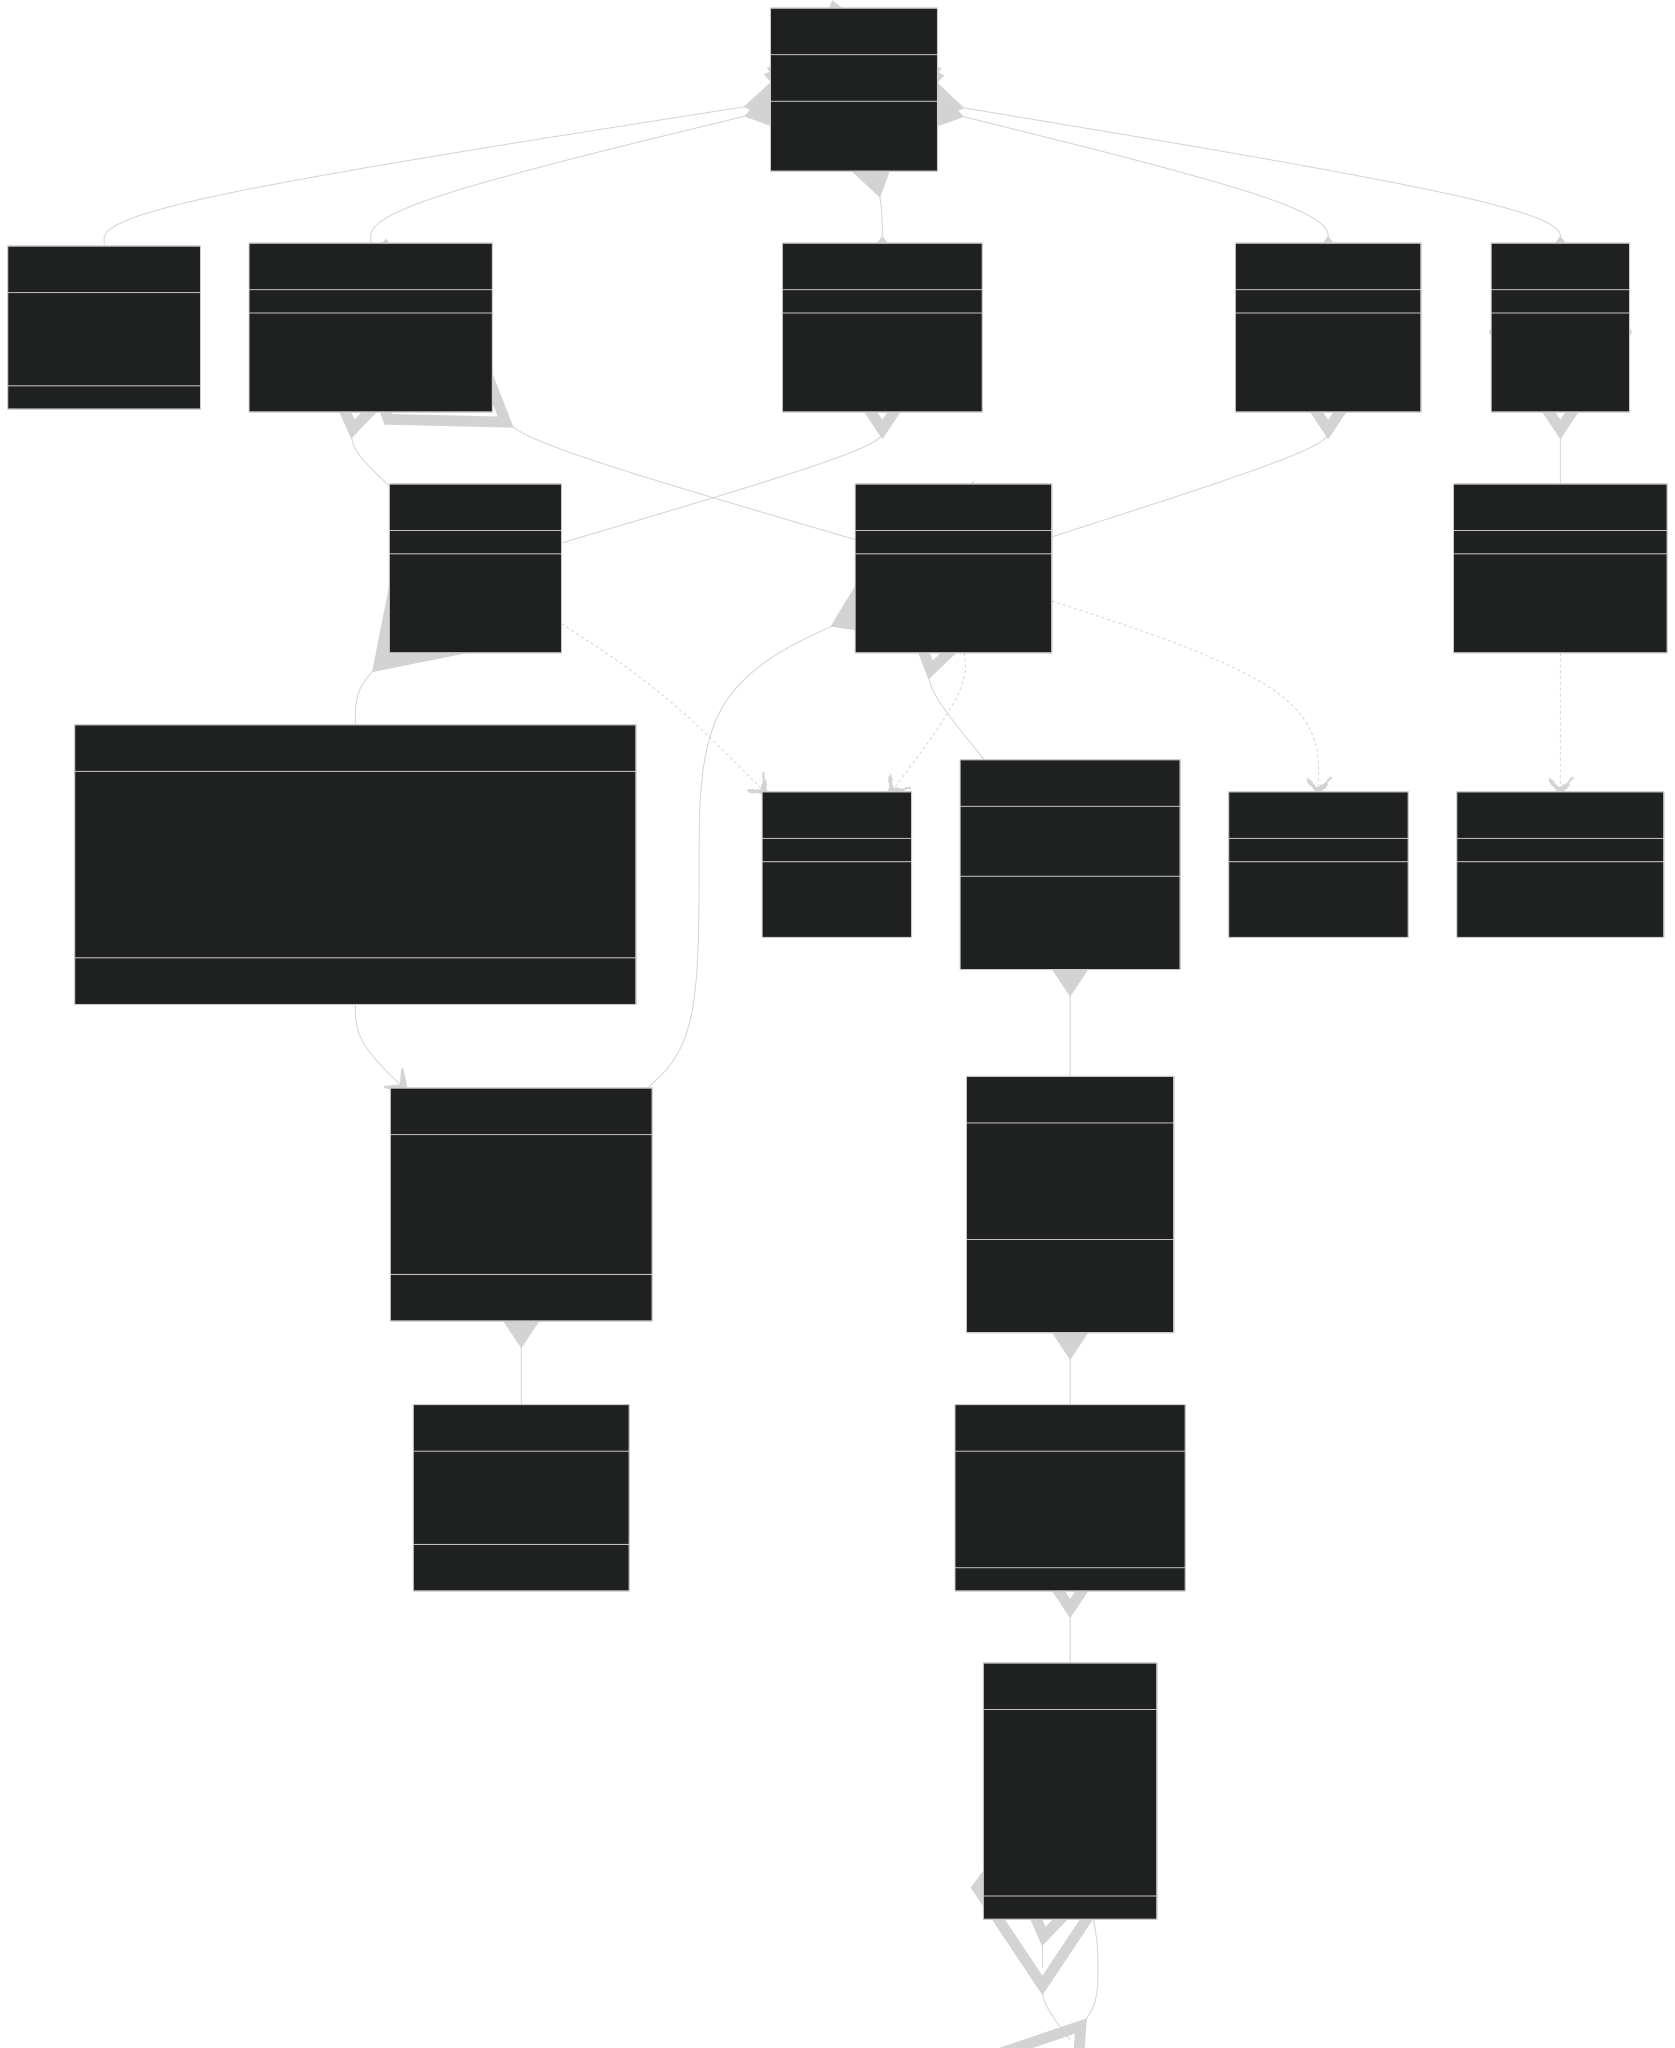
\includegraphics[width=1.1\textwidth, angle=90]{images/diagrama_clases.png}
    \caption{Diagrama de Clases de IPCArt-Studio.}
    \label{fig:diagrama_clases}
\end{figure}


\clearpage

\begin{multicols}{2}


    \section*{Resultados y Discusión}
    La implementación de IPCArt-Studio como una aplicación web moderna ha permitido alcanzar los siguientes resultados:

    \begin{itemize}
        \item Accesibilidad global mediante navegador web
        \item Procesamiento eficiente de imágenes
        \item Gestión robusta de usuarios
        \item Visualización efectiva de estadísticas
        \item Persistencia portable mediante XML
    \end{itemize}

    La arquitectura cliente-servidor implementada permite una clara separación de responsabilidades, facilitando el mantenimiento y la escalabilidad del sistema. El uso de Flask para el backend proporciona una base sólida para la implementación de servicios REST, mientras que Django en el frontend permite una experiencia de usuario fluida y responsive.

    \section*{Conclusiones}
    \begin{itemize}
        \item La implementación de una API REST utilizando Flask proporciona una base sólida para la comunicación cliente-servidor.
        \item El uso de Django para el frontend permite una experiencia de usuario moderna y accesible.
        \item La persistencia mediante XML ofrece una solución portable y mantenible.
        \item El procesamiento de imágenes mediante matrices dispersas optimiza el uso de recursos.
        \item La arquitectura implementada facilita la escalabilidad y mantenimiento del sistema.
    \end{itemize}

    \section*{Referencias}
    \begin{itemize}
        \item Flask Documentation (2024). \textit{Flask Web Development, one drop at a time}. Pallets Projects.
        \item Django Documentation (2024). \textit{The Web framework for perfectionists with deadlines}. Django Software Foundation.
        \item Grinberg, M. (2023). \textit{Flask Web Development: Developing Web Applications with Python}. O'Reilly Media.
        \item Holovaty, A., \& Kaplan-Moss, J. (2024). \textit{The Definitive Guide to Django}. Apress.
    \end{itemize}

\end{multicols}

\end{document}